\vspace{-3pt}
\section{The Electromagnetic Calorimeter}\label{sec:ch3:ecal}

\begin{figure}[h]
\centering
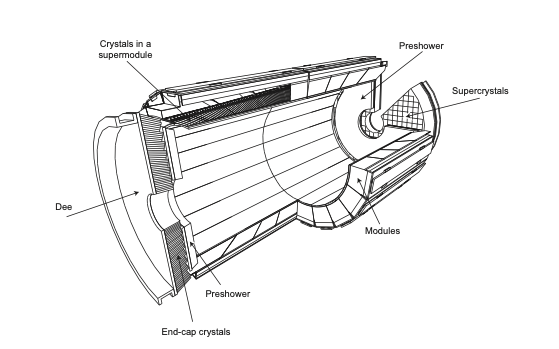
\includegraphics[width=1.0\textwidth]{figures/ecal_replace.png}
\caption{Schematic of the ECAL.}
\label{fig:ECAL}
\end{figure}


The Electromagnetic Calorimeter (ECAL) surrounds the tracker. Its purpose is to absorb the energy from electrons and photons, and was built with the motivation of detecting the decay of two photons for Higgs boson searches. The ECAL is composed of thousands of lead tungstate (PbWO$_4$) crystals, which are mounted on a barrel layer and two endcaps. Before the endcaps, a preshower made of two planes of lead reduces false signals. The schematic of the ECAL can be seen in Figure~\ref{fig:ECAL}.

Lead tungstate crystals are useful in a compact detector because they are radiation-hard and have a small radiation length and small Moliere radius. Additionally, the scintillation decay time of lead tungstate is approximately 25ns, which is the same as the bunch crossing separation in the LHC. The barrel receives the particle data through avalanche photodiodes, which apply a reverse bias voltage to get a current gain effect of about 50. The endcaps use vacuum phototriodes, which are photomultipliers with a single gain state. The vacuum phototriodes usee in the ECAL were developed specifically for CMS, and are useful in the endcaps because they are more radiation resistant than diodes.

The barrel of the ECAL covers $|\eta| < 1.479$, and the endcaps cover $1.479 < |\eta| < 3.0 $. Water cools the submodules containing the crystals at a temperature of 18$^{\circ}$C.


The energy resolution in the ECAL is described by Equation \ref{eq:ecal1}.

\begin{equation}
\left( \frac{\sigma}{E} \right)^2 = \left( \frac{S}{\sqrt{E}} + \left( \frac{N}{E} \right)^2\right)^2 + C^2
\label{eq:ecal1}
\end{equation}

$S$ is the stochastic term, and is comprised of photostatistics (about 2.1\%), fluctuations in energy deposited in the preshower (about 5\%/$\sqrt{E}$), and fluctuations in the lateral shower containment (about 1.5\%). $N$ is the noise term, and is comprised of electronics, digitization, and pileup noise. $C$ is the constant term, and is made up of leakage from the back of the crystals, intercalibration errors, and non-uniformity in light collection, the last being less than a 0.3\% contribution.
